% report.tex

\documentclass[a4paper,11pt]{article}
\usepackage{hyperref}

% Import packages
\usepackage[a4paper]{geometry}
\usepackage[utf8]{inputenc}
\usepackage{amsmath}
\usepackage{amssymb}
\usepackage{enumerate}

\usepackage{graphicx}

\usepackage{listings}


% Change enumerate environments you use letters
\renewcommand{\theenumi}{\alph{enumi}}

% Set title, author name and date
\title{Chitty-Chat}
\author{Johannes Jørgensen, Kevin Skovgaard Gravesen} 
\date{\today}

\begin{document} 

\maketitle

\subsection*{Introduction}
Chitty-Chat is a chat-service that allows clients to communicate via text based messaged through a server. The program is created in the goland programming language with the use of GRPC.
The program uses the command line interface, that allows the clients to write and read between all clients connected to the server.
A broadcast is sent to every connected client when a new client connects, including the new client.

\subsection*{Streaming in Chitty-Chat}
This version of Chitty-Chat is implemented using bidirectional streaming. Which allows for messages to be sent over a single stream.
Every message include the author who send said message. When a message goes from the client only the id is sent, but is changed to the name when the server broadcasts.

Chitty-Chat could also be implemented using server-side streaming with an publish endpoint.
A client could then subscribe to the message stream, where the server will send (broadcast) the published messages.
Another service endpoint would then be used to publish the messages.
This would also allow for different Author signup and TextMessage types in the proto file, where the first text message currently is handled as is if it were an author.

\subsection*{Describe your system architecture - do you have a server-client architecture, peer-to-peer, or something else?}
We have implemented our Chitty-Chat program throught the server-client architecture. 
This means that a server is launched and is only responsible for the communication between different clients. This means that the clients are only responsible for
sending acceptable data from the client to the server.

\subsection*{Describe what  RPC methods are implemented, of what type, and what messages types are used for communication}
We have implemented a single RPC method called \verb|JoinConversation| that both takes and return a \textit{stream} of type \verb|Message|.
The \verb|Message| type is the message type used for communication. It contains the fields:
\begin{itemize}
    \item \verb|timestamp|: A Lamport timestamp
    \item \verb|username|: The username of the sender
    \item \verb|content|: The content of the message
\end{itemize} 

\subsection*{Describe how you have implemented the calculation of the Lamport timestamps}
Both the server and the client have a \verb|Lamport| clock initilized on start, that is set to \verb|0|. This is also the case for newcomers that connect to the server. 
The \verb|Lamport| clock is handled with these conditions:\\
\textbf{Client:}
\begin{itemize}
    \item When a client sends a message, the \verb|Lamport| clock is incremented by \verb|1|.
    \item When a client receives a message, the \verb|Lamport| clock is incremented by \verb|1| if the timestamp of the received message is greater than the current \verb|Lamport| clock.
\end{itemize}
\textbf{Server:}
\begin{itemize}
    \item When the server receives a message, the \verb|Lamport| clock is incremented by \verb|1| if the timestamp of the received message is greater than the current \verb|Lamport| clock.
    \item When the server broadcasts a message, the \verb|Lamport| will be incremented by \verb|1|.
    \item If a client disconnectes from the server, \verb|Lamport| clock is incremented by \verb|1| - Then the server will broadcast the disconnection.
    \item If a client connects to the server, \verb|Lamport| clock is incremented by \verb|1|- Then the server will broadcast the disconnection.
\end{itemize}

\subsection*{Provide a diagram, that traces a sequence of RPC calls together with the Lamport timestamps}
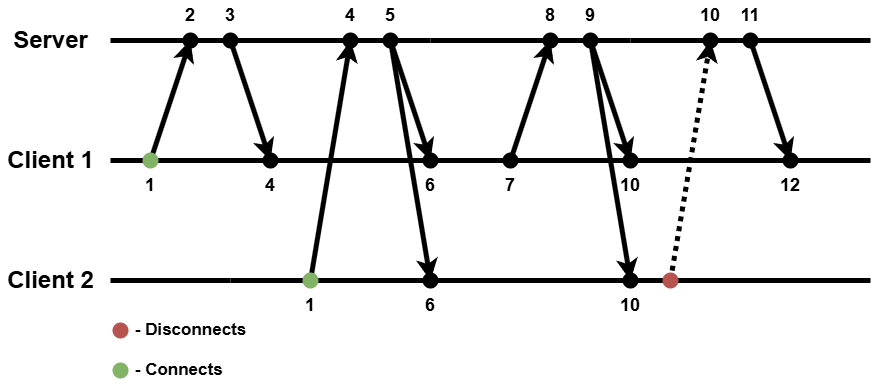
\includegraphics[width=\textwidth]{chat.png}
\begin{enumerate}
        \setlength{\itemsep}{1pt}
        \setlength{\parskip}{0pt}
        \item[1 - \textbf{Server \;}]Starting
        \item[2 - \textbf{Client 1}] Joined the conversation
        \item[3 - \textbf{Client 2}] Joined the conversation
        \item[4 - \textbf{Client 1}] Sends a message
        \item[5 - \textbf{Client 2}] Leaves the conversation
    \end{enumerate}

\subsection*{Git}
\href{https://github.com/ITU-DISYS2024-CENTRALIZEDSYSTEMS/Chitty-Chat}{Github}

\subsection*{Appendix}

\subsubsection*{Lamport logs}
\begin{lstlisting}[basicstyle=\ttfamily\footnotesize]
Server:
2024/10/22 14:32:31 Info | Client 1 | Joined Chitty-Chat | Lamport time 2
2024/10/22 14:32:31 Broadcasting | Client 1 | joined Chitty-Chat | Lamport time 3
2024/10/22 14:32:42 Info | Client 2 | Joined Chitty-Chat | Lamport time 4
2024/10/22 14:32:42 Broadcasting | Client 2 | joined Chitty-Chat | Lamport time 5
2024/10/22 14:32:58 Info | Client 1 | Sent a message | Lamport time 8
2024/10/22 14:32:58 Broadcasting | Client 1 | Hello world! | Lamport time 9
2024/10/22 14:33:00 Info | Client 2 | Dropped the connection! | Lamport time 10
2024/10/22 14:33:00 Broadcasting | Client 2 | left Chitty-Chat | Lamport time 12

Client 1:
2024/10/22 14:32:31 Client 1 | joined Chitty-Chat | Lamport time 4
2024/10/22 14:32:42 Client 2 | joined Chitty-Chat | Lamport time 6
2024/10/22 14:32:58 Client 1 | Hello world! | Lamport time 10
2024/10/22 14:33:00 Client 2 | left Chitty-Chat | Lamport time 13

Client 2:
2024/10/22 14:32:42 Client 2 | joined Chitty-Chat | Lamport time 6
2024/10/22 14:32:58 Client 1 | Hello world! | Lamport time 10
\end{lstlisting}

\subsubsection*{Chitty-Chat demo: 5 clients}
\begin{lstlisting}[basicstyle=\ttfamily\footnotesize]
Server:
2024/10/22 14:41:28 Info | Client 1 | Joined Chitty-Chat | Lamport time 2
2024/10/22 14:41:28 Broadcasting | Client 1 | joined Chitty-Chat | Lamport time 3
2024/10/22 14:41:37 Info | Client 2 | Joined Chitty-Chat | Lamport time 4
2024/10/22 14:41:37 Broadcasting | Client 2 | joined Chitty-Chat | Lamport time 5
2024/10/22 14:42:21 Info | Client 3 | Joined Chitty-Chat | Lamport time 6
2024/10/22 14:42:21 Broadcasting | Client 3 | joined Chitty-Chat | Lamport time 7
2024/10/22 14:42:30 Info | Client 4 | Joined Chitty-Chat | Lamport time 8
2024/10/22 14:42:30 Broadcasting | Client 4 | joined Chitty-Chat | Lamport time 9
2024/10/22 14:42:43 Info | Client 5 | Joined Chitty-Chat | Lamport time 10
2024/10/22 14:42:43 Broadcasting | Client 5 | joined Chitty-Chat | Lamport time 11
2024/10/22 14:43:02 Info | Client 1 | Sent a message | Lamport time 14
2024/10/22 14:43:02 Broadcasting | Client 1 | Hello world from 1! | Lamport time 15
2024/10/22 14:43:09 Info | Client 3 | Sent a message | Lamport time 18
2024/10/22 14:43:09 Broadcasting | Client 3 | Hello world from 3! | Lamport time 19
2024/10/22 14:43:12 Info | Client 4 | Sent a message | Lamport time 22
2024/10/22 14:43:12 Broadcasting | Client 4 | Hello world from 4 | Lamport time 23
2024/10/22 14:43:16 Info | Client 5 | Sent a message | Lamport time 26
2024/10/22 14:43:16 Broadcasting | Client 5 | Hello world from 5 | Lamport time 27
2024/10/22 14:43:29 Info | Client 2 | Sent a message | Lamport time 30
2024/10/22 14:43:29 Broadcasting | Client 2 | Hello world from 2! | Lamport time 31

Client 1:
2024/10/22 14:41:28 Client 1 | joined Chitty-Chat | Lamport time 4
2024/10/22 14:41:37 Client 2 | joined Chitty-Chat | Lamport time 6
2024/10/22 14:42:21 Client 3 | joined Chitty-Chat | Lamport time 8
2024/10/22 14:42:30 Client 4 | joined Chitty-Chat | Lamport time 10
2024/10/22 14:42:43 Client 5 | joined Chitty-Chat | Lamport time 12
2024/10/22 14:43:02 Client 1 | Hello world from 1! | Lamport time 16
2024/10/22 14:43:09 Client 3 | Hello world from 3! | Lamport time 20
2024/10/22 14:43:12 Client 4 | Hello world from 4 | Lamport time 24
2024/10/22 14:43:16 Client 5 | Hello world from 5 | Lamport time 28
2024/10/22 14:43:29 Client 2 | Hello world from 2! | Lamport time 32

Client 2:
2024/10/22 14:41:37 Client 2 | joined Chitty-Chat | Lamport time 6
2024/10/22 14:42:21 Client 3 | joined Chitty-Chat | Lamport time 8
2024/10/22 14:42:30 Client 4 | joined Chitty-Chat | Lamport time 10
2024/10/22 14:42:43 Client 5 | joined Chitty-Chat | Lamport time 12
2024/10/22 14:43:02 Client 1 | Hello world from 1! | Lamport time 16
2024/10/22 14:43:09 Client 3 | Hello world from 3! | Lamport time 20
2024/10/22 14:43:12 Client 4 | Hello world from 4 | Lamport time 24
2024/10/22 14:43:16 Client 5 | Hello world from 5 | Lamport time 28
2024/10/22 14:43:29 Client 2 | Hello world from 2! | Lamport time 32

Client 3:
2024/10/22 14:42:21 Client 3 | joined Chitty-Chat | Lamport time 8
2024/10/22 14:42:30 Client 4 | joined Chitty-Chat | Lamport time 10
2024/10/22 14:42:43 Client 5 | joined Chitty-Chat | Lamport time 12
2024/10/22 14:43:02 Client 1 | Hello world from 1! | Lamport time 16
2024/10/22 14:43:09 Client 3 | Hello world from 3! | Lamport time 20
2024/10/22 14:43:12 Client 4 | Hello world from 4 | Lamport time 24
2024/10/22 14:43:16 Client 5 | Hello world from 5 | Lamport time 28
2024/10/22 14:43:29 Client 2 | Hello world from 2! | Lamport time 32

Client 4:
2024/10/22 14:42:30 Client 4 | joined Chitty-Chat | Lamport time 10
2024/10/22 14:42:43 Client 5 | joined Chitty-Chat | Lamport time 12
2024/10/22 14:43:02 Client 1 | Hello world from 1! | Lamport time 16
2024/10/22 14:43:09 Client 3 | Hello world from 3! | Lamport time 20
2024/10/22 14:43:12 Client 4 | Hello world from 4 | Lamport time 24
2024/10/22 14:43:16 Client 5 | Hello world from 5 | Lamport time 28
2024/10/22 14:43:29 Client 2 | Hello world from 2! | Lamport time 32

Client 5:
2024/10/22 14:42:43 Client 5 | joined Chitty-Chat | Lamport time 12
2024/10/22 14:43:02 Client 1 | Hello world from 1! | Lamport time 16
2024/10/22 14:43:09 Client 3 | Hello world from 3! | Lamport time 20
2024/10/22 14:43:12 Client 4 | Hello world from 4 | Lamport time 24
2024/10/22 14:43:16 Client 5 | Hello world from 5 | Lamport time 28
2024/10/22 14:43:29 Client 2 | Hello world from 2! | Lamport time 32
\end{lstlisting}
\end{document}